\documentclass[journal,10pt]{IEEEtran}
\usepackage[T1]{fontenc}
\usepackage{mathptmx}
\usepackage{amsmath,amssymb,booktabs,array,multirow}
\usepackage{graphicx,xcolor}
\usepackage{algorithm,algpseudocode}
\usepackage{cite,url}
\usepackage[hidelinks]{hyperref}
\usepackage{placeins,balance}
\definecolor{draftink}{RGB}{66,79,97}
\newcommand{\LEAF}{\textsc{LEAF}}
\newcommand{\draftfigure}[2]{%
  \begin{figure}[t]\centering
  \setlength{\fboxsep}{10pt}%
  \fcolorbox{draftink!35}{draftink!3}{%
  \begin{minipage}{\dimexpr\columnwidth-2\fboxsep-2\fboxrule\relax}
  \small\color{draftink}\textbf{Figure slot: #1}\par\medskip
  #2\par\medskip
  \textit{Reserved for the next visual iteration.}
  \end{minipage}}
  \caption{Planned evidence display: #1.}\end{figure}}
\hyphenation{multi-agent gene-ra-li-za-tion re-pre-sen-ta-tion}
\hypersetup{pdftitle={LEAF: Looped Entity Attention Fusion -- Initial Draft},pdfauthor={}}
\begin{document}
\title{LEAF: Looped Entity Attention Fusion for Scale-Generalizable Multi-Agent Defense}
\author{Anonymous Authors}
\bstctlcite{leafBibliographyControl}
\maketitle
\markboth{LEAF: Working Draft -- Experimental Figure Slots Open}{LEAF: Working Draft}
\begin{abstract}
Cooperative target protection requires a shared policy to coordinate defenders as vehicle populations and protected targets change. We study frozen-policy transfer across these changes against a fixed reactive attacker controller. We present Looped Entity Attention Fusion (LEAF), which repeatedly updates receiver-relative entity representations with a shared attention block. Each defender uses its own state and temporal memory to read and fuse intermediate representations before selecting an action. Sampled-depth training couples short and long computation paths within entity-factorized value learning. In simulation, LEAF improves target protection across population shifts relative to REFIL and yields a more effective one-round policy than independent one-round training. Representation probes reveal accessible geometric threat information, while frozen-policy interventions show that early reads and temporal memory influence decisions. These findings support shared iterative processing with individual access to intermediate information for cooperative control across changing populations.
\end{abstract}
\noindent\textbf{Note to Practitioners---}
Protection systems often operate with changing numbers of vehicles and assets, creating a practical need for controllers that can be reused across engagement configurations. This work develops a shared controller that processes entity states, refines their interaction information, and reads the resulting representations from each defender's perspective. An individual memory state supplies temporal context. The controller learns in small simulated engagements and is evaluated with frozen parameters under larger vehicle populations and additional targets. Accumulated target damage measures protection quality. Applying this interface requires estimates of entity positions and velocities, a compatible action interface, and a recurrent state for each defender. The unfolding depth specifies the number of entity updates performed at each decision. For a physical platform, the corresponding control cycle can be selected using measured inference time together with protection performance under the platform's sensing and motion conditions.
\begin{IEEEkeywords}
Multi-agent reinforcement learning, cooperative control, scale generalization, entity attention, target protection.
\end{IEEEkeywords}

\section{Introduction}
\IEEEPARstart{C}{ooperative} target protection requires defenders to redistribute their effort as the numbers of vehicles and protected assets change. An attacker approaching a target may already be covered by a well-positioned teammate, while another attacker threatens an exposed asset. Effective actions therefore depend on relationships among attackers, targets, and defenders, interpreted from the perspective of the defender choosing an action. Increasing team size or target count changes these relationships and the distribution of responsibilities. A shared controller that carries useful interaction patterns across engagement sizes would simplify deployment across changing configurations.

Entity-based policies provide a common interface to these changing scenes. Shared encoders and attention accommodate variable entity populations, while REFIL encourages reuse of interaction patterns through randomized entity-wise value factorization~\cite{iqbal2021refil}. Individual decisions also involve two connected computations: developing an entity's context and extracting information relevant to the receiving defender. An attacker's representation can incorporate its relationships to targets and teammates; its relevance to a particular action depends on the defender's own state and history. In the task studied here, public physical states describe the scene, while the attacker's private target assignment gives recent motion a role in interpreting that scene.

Shared iterative attention offers a reusable operator for developing entity context. Relational reinforcement learning and Universal Transformers establish repeated processing with shared attention parameters~\cite{zambaldi2019relational,dehghani2019universal}. Each fully connected update accesses the permitted entity set, and subsequent updates process the context formed by earlier applications. Preserving intermediate states gives the decision stage access to several stages of this computation, following the broader principle of combining representations across depth~\cite{xu2018jk}. Figure~\ref{fig:motivation} illustrates the resulting design idea: develop entity context and make its intermediate representations available to an individualized reader.

We introduce \textbf{Looped Entity Attention Fusion (LEAF)}, which connects shared entity refinement to individual action selection through history-conditioned reading and learned cross-round fusion. Each defender initializes a receiver-relative entity workspace and repeatedly applies one shared attention block. A query constructed from its initial self representation and previous temporal memory reads every intermediate entity set. Learned weights combine these summaries, and a residual projection adds the fused information to the feature entering a recurrent utility network. The network then performs one temporal update and produces action values. Figure~\ref{fig:framework} shows how within-step refinement connects to the memory carried between physical decisions.

Training samples the unfolding depth while retaining REFIL's entity-factorized cooperative learning objective. Early representations directly supply the reader and also become inputs to subsequent updates at longer unfoldings. The same policy parameters therefore learn through both short decision paths and longer sequences of entity processing. Training across depths has a related precedent in LayerDrop~\cite{fan2020layerdrop}; LEAF uses different unfolding lengths of a shared operator with access to the resulting intermediate states. This design motivates evaluating the quality of a learned one-round policy alongside the effects of additional execution rounds and different readout choices.

We evaluate frozen-policy transfer across team-size, target-count, and joint changes in simulated protection against a fixed reactive attacker controller (Fig.~\ref{fig:scenario}). LEAF improves protection relative to REFIL across the evaluated population shifts. Matched one-round execution supports a more effective policy after multi-depth training, while frozen-policy interventions connect the learned decisions to early reads and temporal conditioning. Representation probes further examine the geometric information accessible in the entity states. The contributions are:
\begin{enumerate}
\item A shared refinement and individual readout architecture that connects intermediate entity states to recurrent action values.
\item A sampled-depth learning design that couples short and long unfoldings within entity-factorized value learning.
\item A population-transfer evaluation with matched-depth comparisons and targeted interventions on intermediate reads and temporal conditioning.
\end{enumerate}

\begin{figure*}[t]
\centering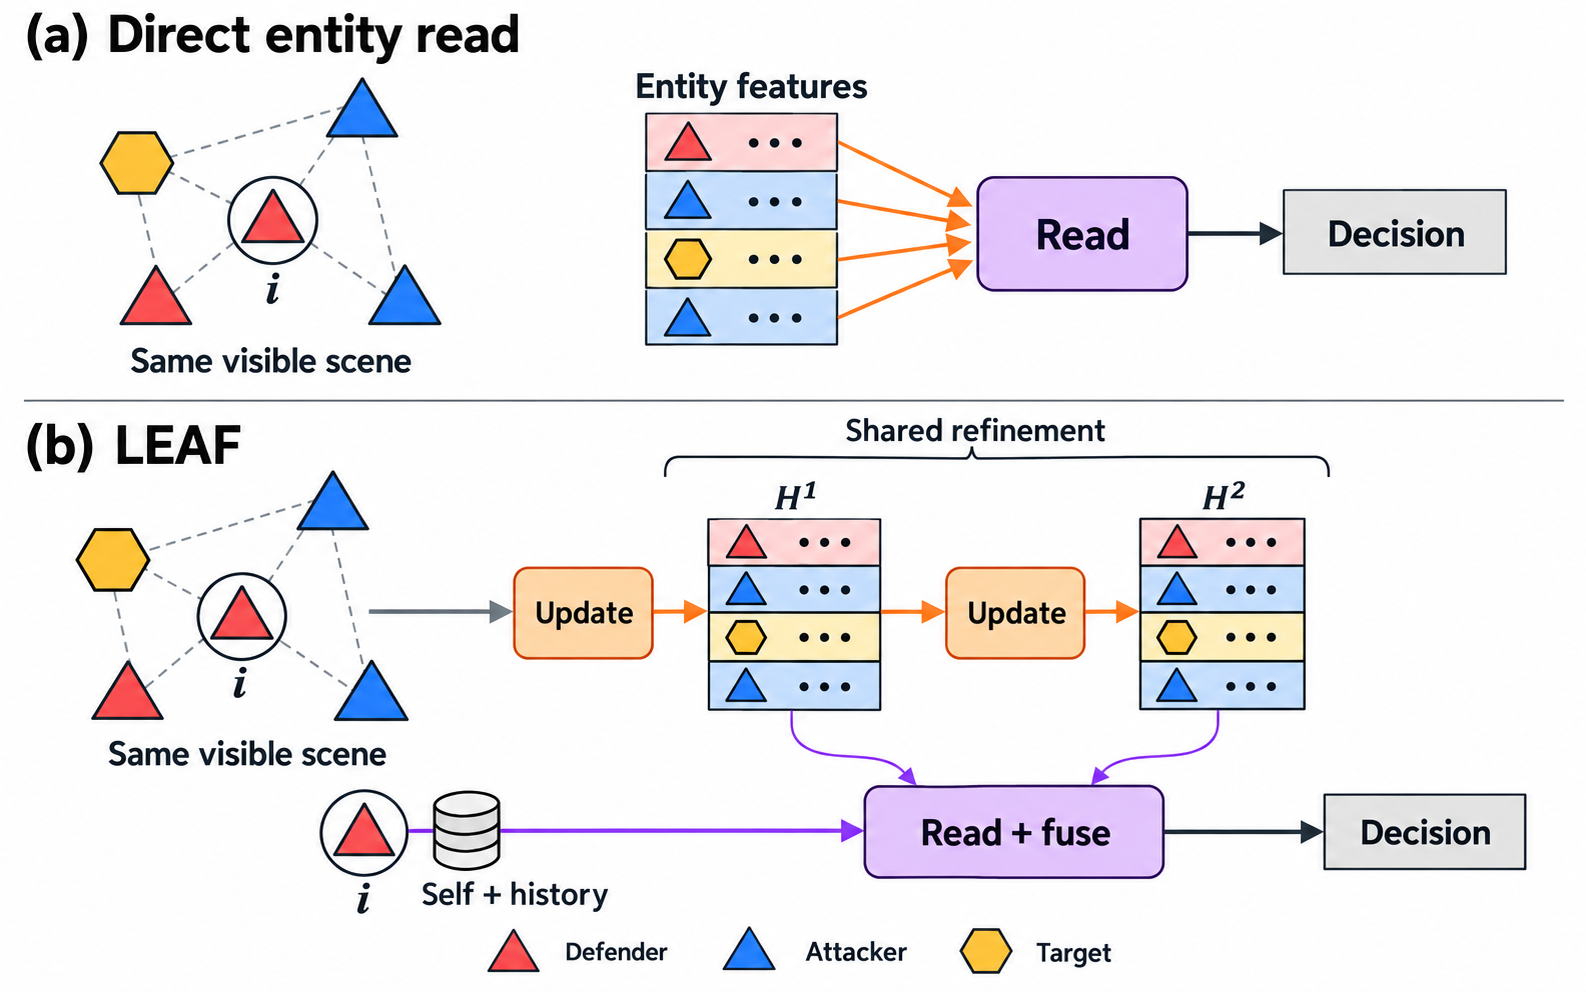
\includegraphics[width=.94\textwidth]{figures/fig1_motivation.png}
\caption{Entity processing for individual decisions. A direct entity read aggregates encoded features for action selection. LEAF develops entity context through shared refinement and gives each defender access to intermediate representations through a self- and history-conditioned reader. Both paths receive the same visible scene; the illustrated updates occur within one decision step. Entity rows are schematic.}
\label{fig:motivation}
\end{figure*}
\section{Related Work}
\subsection{Entity-Based Policies for Changing Populations}
Set representations and attention provide reusable interfaces for variable entity populations~\cite{zaheer2017deepsets,lee2019settransformer}. In cooperative learning, REFIL combines entity attention with randomized entity partitions and an auxiliary factorized value objective~\cite{iqbal2021refil}. LEAF retains this learning foundation and develops the path from entity encoding to recurrent utilities. Related architectures address complementary parts of this interface: UPDeT connects variable observations and action configurations~\cite{hu2021updet}, TransfQMix uses transformers in agent and mixing networks~\cite{transfqmix2023}, and SPECTra combines observer-conditioned reading with scalable value mixing~\cite{park2026spectra}. These connections place LEAF's contribution in the joint use of contextual entity updates and individualized access to their intermediate states.

\subsection{Shared Refinement and Access Across Depth}
Zambaldi et al. establish shared iterative relational attention in reinforcement learning~\cite{zambaldi2019relational}, and Universal Transformers reuse a self-attentive transition across processing depth~\cite{dehghani2019universal}. Jumping Knowledge networks combine intermediate representations to adapt their use to the receiving node~\cite{xu2018jk}. LayerDrop trains with sampled transformer-layer subsets and supports shallow execution paths~\cite{fan2020layerdrop}. LEAF combines these principles through sampled unfoldings of one shared entity operator and a common reader that accesses every retained round. The receiver's temporal memory conditions this reading, linking within-step refinement to the recurrent utility network. Its evaluation separately examines training depth, execution depth, and intermediate-information use.

\subsection{Cooperative Protection and Automation}
Cooperative control couples threat response with the allocation of team effort. Recent automation studies examine hierarchical allocation and motion planning for swarm confrontation~\cite{wu2025swarm}, observer-assisted pursuit under uncertainty~\cite{liu2025observer}, and scalable aircraft separation assurance~\cite{brittain2022separation}. These tasks motivate controllers that remain useful as interactions and operating configurations change. LEAF studies this deployment requirement through one defender policy evaluated across vehicle and protected-target populations, with physical rules and a reactive opponent held fixed.

\begin{figure*}[t]
\centering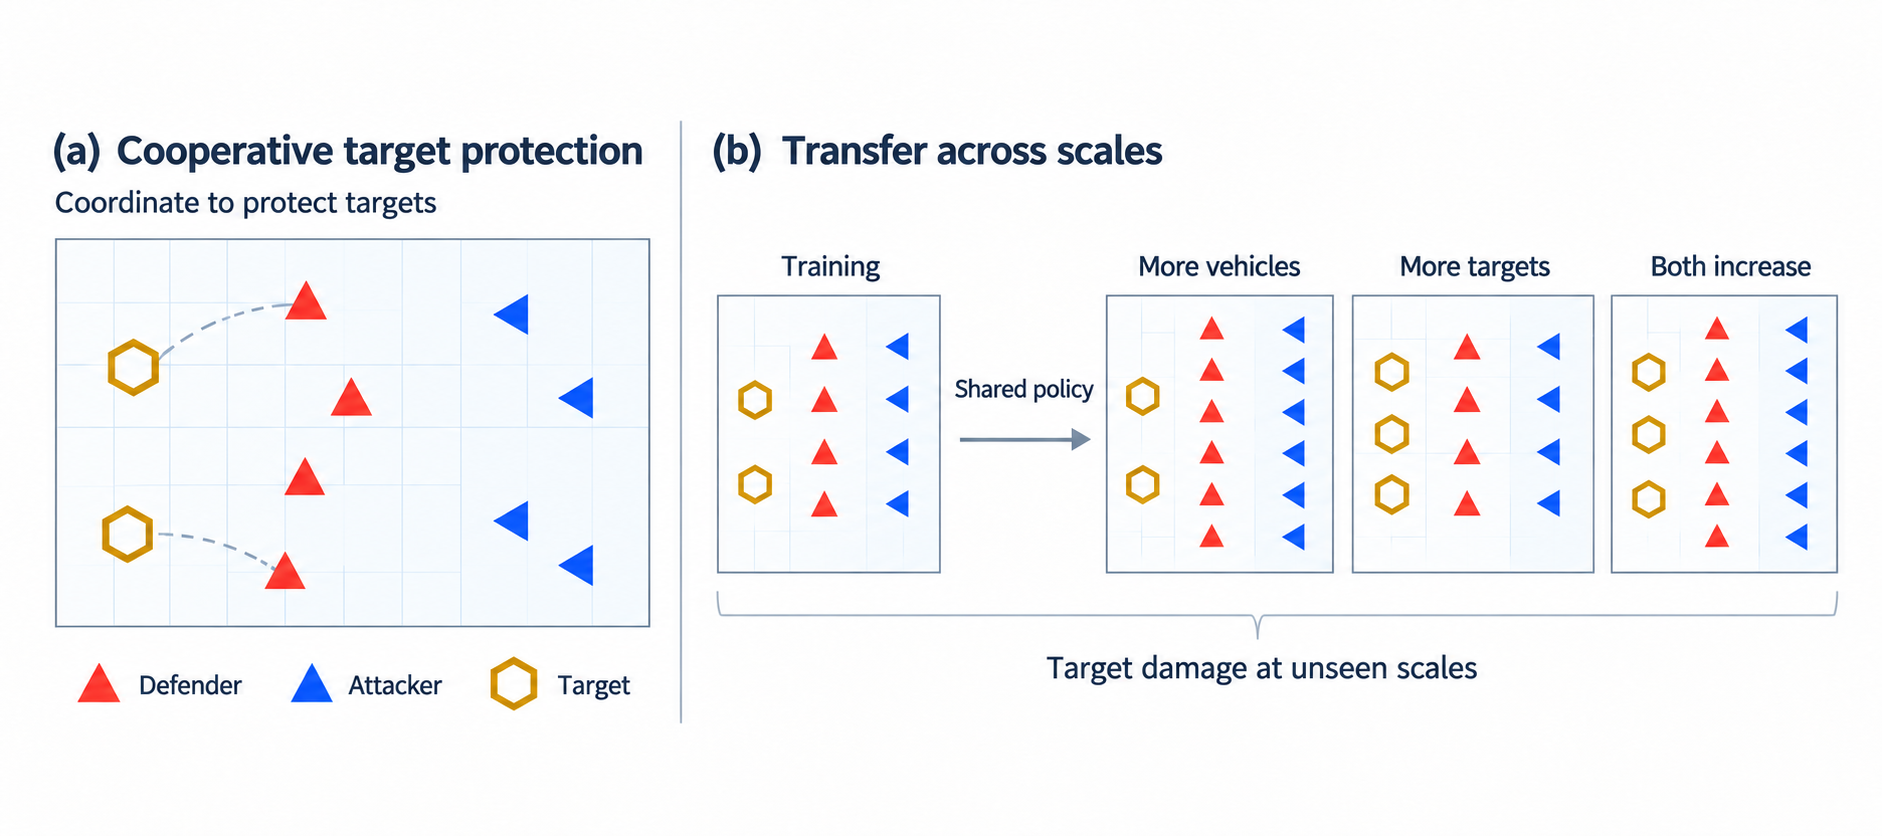
\includegraphics[width=\textwidth]{figures/fig2_scenario.png}
\caption{Cooperative target protection across population changes. A shared defender policy learns in small engagements and is evaluated with frozen parameters as vehicle populations, target populations, or both increase. Icon counts illustrate the three types of change; the training and evaluation configurations are defined in the experimental protocol. The background grid is a visual guide to the continuous arena.}
\label{fig:scenario}
\end{figure*}
\section{Problem Formulation and Preliminaries}
\label{sec:problem}
\subsection{Cooperative Target Protection}
We study a planar attack--defense simulator (HAD) in which defenders coordinate their actions against incoming attackers across a changing set of protected targets. Let $\mathcal R$, $\mathcal B$, and $\mathcal T$ denote the defender, attacker, and target sets, with initial configuration $\mathbf n=(N_R,N_B,K)$. Targets occupy the left portion of the arena; attackers approach from the right, and defenders distribute their responses between interception and target coverage. Figure~\ref{fig:scenario} illustrates the task and its population changes.

Vehicles choose among eight normalized acceleration directions and zero acceleration. Close vehicle encounters can remove both participants, while automatic firing allows defenders to engage attackers and attackers to damage targets. Targets remain as damage accumulates. The simulator continues after the final defender disappears and ends when all attackers have disappeared or the episode horizon is reached. Table~\ref{tab:environment} collects the physical interface used by all policies.

\begin{table}[t]
\centering\footnotesize
\caption{HAD physical interface. Damage-event ordering and terminal reward handling follow the common simulator.}
\label{tab:environment}
\begin{tabular}{@{}ll@{}}\toprule
Quantity & Setting\\\midrule
Arena & $5000\times5000$ m\\
Decision interval / horizon & 1 s / 100 steps\\
Acceleration limit & $40\,\mathrm{m/s^2}$\\
Vehicle speed range & $35$--$120\,\mathrm{m/s}$\\
Swept collision distance & 20 m\\
Automatic firing separation & Below 200 m, pre-movement\\
Damage profile & Unit core to 200 m; linear to 0 at 400 m\\
\bottomrule\end{tabular}
\end{table}

Public observations contain entity positions, velocities, types, health or alive status, and target damage. The fixed reactive attacker controller selects a target using public defender coverage and distances, then carries out a rush and periodically revises its assignment. That assignment is private. Recent motion therefore provides useful context for interpreting the attackers' evolving objectives.

Let $\Delta d_{k,t}$ be damage to target $k$ at step $t$. Physical reward and evaluation damage are
\begin{equation}
\Delta D_t=\sum_{k\in\mathcal T}\Delta d_{k,t},\qquad
r_t=-\Delta D_t,\qquad D=\sum_t\Delta D_t.
\label{eq:damage}
\end{equation}
Lower accumulated damage indicates better protection. Comparisons use identical configurations and initial-scene conditions.

\subsection{Population Generalization}
With the attacker controller $\pi_B$ fixed, the team faces a family of cooperative partially observable decision processes indexed by $\mathbf n$. Defender $i$ acts from its observation--action history $\tau_{i,t}$ through a shared policy $\pi_\theta$, maintaining its own temporal state. The latent state includes the private attacker assignment.

Training samples small engagements. Evaluation freezes $\theta$ and varies vehicle populations, target populations, or both, while retaining the physical rules, action semantics, and attacker controller. The quantity of interest is $\mathbb E[D\mid\mathbf n,\pi_\theta,\pi_B]$ across held-out configurations. This formulation connects population transfer to a concrete control requirement: distributing defensive responses among a changing set of interacting entities.

\subsection{Entity-Factorized Cooperative Learning}
LEAF builds on REFIL's entity-based utility network and imagined decomposition~\cite{iqbal2021refil}. A shared encoder and masked attention produce a base feature $\ell_{i,t}$ for each defender. A recurrent utility network combines that feature with individual memory to produce $Q_i(\tau_{i,t},a_{i,t})$. Centralized training uses a scene-conditioned monotonic mixer,
\begin{equation}
Q_{\mathrm{tot}}(x_t,\boldsymbol a_t)=f_{\mathrm{mix}}(Q_1,\ldots,Q_{N_R};x_t),
\quad\frac{\partial Q_{\mathrm{tot}}}{\partial Q_i}\geq0,
\end{equation}
so individual greedy actions are consistent with a maximizer of the represented joint value over legal action sets~\cite{rashid2018qmix}.

REFIL draws random entity partitions and forms in-group and out-group masked views of each recorded sequence. These views produce an auxiliary team value that shares the main branch's temporal-difference target. LEAF retains this learning interface and augments the feature entering the recurrent utility network. Each branch applies its entity mask and reconstructs its temporal history with shared parameters. Deployment uses the main branch.

\begin{figure*}[t]
\centering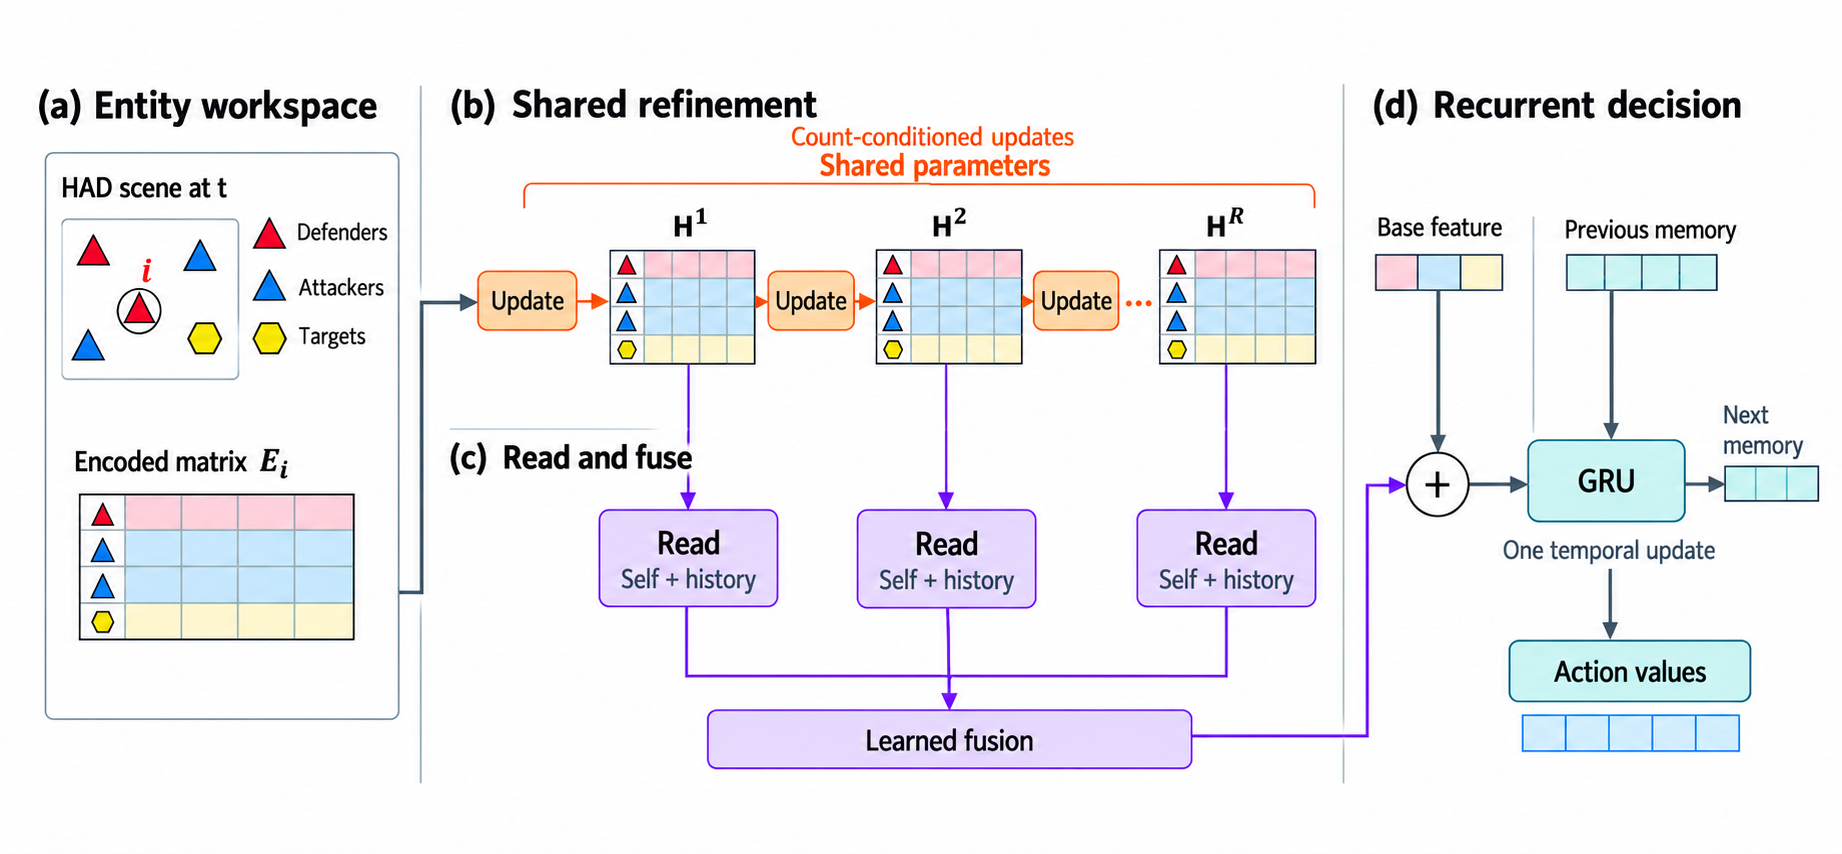
\includegraphics[width=\textwidth]{figures/fig3_framework.png}
\caption{LEAF at one defender decision. Shared, count-conditioned attention updates a receiver-relative entity workspace. One query, formed from the initial self token and a stop-gradient copy of previous temporal memory, reads every intermediate set. Learned fusion is projected and added to the base feature before one GRU update produces the next memory and action values. Update and readout parameters are reused across rounds; the next observation initializes a fresh workspace. Entity rows and feature cells are schematic.}
\label{fig:framework}
\end{figure*}
\section{Looped Entity Attention Fusion}
\label{sec:method}
LEAF repeatedly updates a receiver-relative entity set with one shared attention block, reads every intermediate set using the defender's self representation and temporal memory, and fuses the reads before updating the recurrent utility network. Figure~\ref{fig:framework} gives the complete information flow.

\subsection{Receiver-Relative Entity Workspace}
At time $t$, defender $i$ receives an entity matrix $X_{i,t}$ and a mask $m_{i,t,e}\in\{0,1\}$ indicating permitted key rows. The main branch uses the public entities, while imagined branches impose their additional partition masks. Other entities are encoded relative to defender $i$; its self row retains absolute features. Inputs contain normalized planar positions and velocities, alive/health information, target damage, entity type, and previous-action features. A shared encoder gives entity embeddings $e_{i,t,e}$ and the REFIL feature $\ell_{i,t}$.

The LEAF workspace has width $d=64$. On valid rows its initial representation is
\begin{equation}
 H^{(0)}_{i,t,e}=W_g e_{i,t,e}+b_g.
 \label{eq:workspace}
\end{equation}
The projected self token is retained for query construction under the branch convention, and entity interactions use the permitted-key mask. Excluded rows have no key contribution and are zeroed after each shared update. Each defender thus has a receiver-relative workspace, with common network parameters across defenders and branches. A new observation initializes a new workspace.

Population information enters through a bounded typed-count encoding. Let $n_R$, $n_B$, and $n_T$ be the numbers of permitted defenders, attackers, and targets under the current mask. Define
\begin{align}
 \rho(n)&=\left[\left(\frac{(n-1)_+}{(n-1)_++2}\right)^2,
                   \mathbb I[n=0]\right],\nonumber\\
 z_i&=\operatorname{MLP}\bigl([\rho(n_R);\rho(n_B);\rho(n_T)]\bigr),
 \label{eq:counts}
\end{align}
where $(v)_+=\max(v,0)$ and $\mathbb I[\cdot]$ is an indicator. The first coordinate summarizes increasing population size, and the second distinguishes an empty set from a singleton. This encoding conditions the entity-update queries. Typed-count injection is enabled in all evaluated LEAF checkpoints.

\subsection{Repeated Contextual Entity Updates}
Suppressing defender, time, and branch indices, one round applies
\begin{align}
 J^{(r)}&=\operatorname{LN}_a(H^{(r-1)})
              +\mathbf1(W_cz+b_c)^\top,\nonumber\\
 \widetilde H^{(r)}&=H^{(r-1)}
       +\operatorname{MHA}_{\theta}(J^{(r)},H^{(r-1)},H^{(r-1)};m),\nonumber\\
 H^{(r)}&=\operatorname{Mask}_{m}\!\left[\widetilde H^{(r)}
       +\operatorname{FFN}_{\theta}
                  (\operatorname{LN}_f(\widetilde H^{(r)}))\right].
 \label{eq:loop}
\end{align}
Here $\operatorname{LN}$ denotes rowwise layer normalization, $\operatorname{MHA}(Q,K,V;m)$ is masked multihead attention, and $\operatorname{Mask}_m$ zeros excluded rows. The vector $\mathbf1$ broadcasts the count feature over entity queries. An empty permitted-key set returns a zero attention aggregate. The same update parameters are reused for $r=1,\ldots,R$. Keys and values at round $r$ are the representations from round $r-1$, so the operator acts on the context produced by its preceding application.

Within the permitted set, attention connects every valid entity to every other valid entity from the first round onward. Later rounds therefore refine already contextualized features. Entity rows retain their identities, and every intermediate set $H^{(1)},\ldots,H^{(R)}$ remains available to the reader. This organization follows shared relational processing~\cite{zambaldi2019relational,dehghani2019universal} and gives the decision stage access to several stages of that processing. The anchored-key/value comparator ARR instead supplies $H^{(0)}$ as keys and values at each update.

\subsection{History-Conditioned Reading and Fusion}
The receiver constructs one query from its initial self token and previous temporal memory:
\begin{align}
 q_{i,t}&=W_q[H^{(0)}_{i,t,\mathrm{self}};
                    \operatorname{sg}(h_{i,t-1})]+b_q,\nonumber\\
 u_{i,t}^{(r)}&=\operatorname{MHA}_{\mathrm{read}}
                  (q_{i,t},H_{i,t}^{(r)},H_{i,t}^{(r)};m_{i,t}).
 \label{eq:read}
\end{align}
The readout $u_{i,t}^{(r)}\in\mathbb R^{64}$ summarizes round $r$ for defender $i$. The same query and reader parameters are used for every round at the current decision. Each read attends directly to its corresponding entity set. The stop-gradient operator $\operatorname{sg}$ preserves the forward value of the GRU state and blocks the gradient through its query-input copy. Backpropagation through the GRU's temporal recurrence remains active. This query stop-gradient is used by every evaluated LEAF checkpoint.

A shared scalar scoring map assigns weights to the available reads:
\begin{equation}
 \alpha_{i,t}^{(r)}=
 \frac{\exp(w_s^\top u_{i,t}^{(r)}+b_s)}
 {\sum_{j=1}^{R}\exp(w_s^\top u_{i,t}^{(j)}+b_s)},\qquad
 u_{i,t}=\sum_{r=1}^{R}\alpha_{i,t}^{(r)}u_{i,t}^{(r)}.
 \label{eq:fusion}
\end{equation}
These nonnegative weights sum to one. Entity attention within a round determines what the defender reads, and cross-round fusion determines how those summaries contribute to its decision feature. Both depend on the receiver through its self state and memory. Preserving intermediate representations supports selection across processing depth~\cite{xu2018jk}; the learned scores determine their contribution in each observed situation.

The fused read augments the REFIL feature through a residual projection:
\begin{align}
 \ell'_{i,t}&=\ell_{i,t}+W_f u_{i,t}+b_f,\nonumber\\
 h_{i,t}&=\operatorname{GRU}(\ell'_{i,t},h_{i,t-1}),\nonumber\\
 Q_i(\tau_{i,t},\cdot)&=W_o h_{i,t}+b_o.
 \label{eq:decision}
\end{align}
The projection $W_fu+b_f$ is initialized to zero, so learning starts from the original feature path and jointly adapts both paths thereafter. Each branch updates the GRU once per defender decision at a physical time step. Its hidden state persists to the next observation, while the entity workspace is rebuilt from that observation. Thus $r$ indexes repeated computation at one decision and $t$ indexes physical evolution. All rounds are computed before fusion; small fusion weights affect information use while the chosen depth $R$ determines the computation performed.



\subsection{Learning Across Processing Depths}
Collection samples $R$ uniformly from $\{1,2,3,4\}$ and holds it fixed for an episode. Replay independently samples one depth per training batch and uses that depth for the online main and imagined branches and the target network. At depth one, the shared update directly supplies the value objective. At larger depths, its output also becomes the input to subsequent applications. Consequently, the same parameters learn through both short decision paths and longer sequences of contextual updates. Standard deployment fixes $R=4$.

Learning retains the shared potential-shaped reward used by the REFIL host:
\begin{align}
 \widetilde r_t&=-\Delta D_t+\gamma\Phi(s_{t+1})-\Phi(s_t),\nonumber\\
 \Phi(s)&=-\sum_{j\in\mathcal B_{\mathrm{alive}}}
 \operatorname{clip}\!\left(1-\frac{\min_{k\in\mathcal T}\|p_j-p_k\|}{4000},0,1\right),
 \label{eq:shaping}
\end{align}
where $p_j$ and $p_k$ are attacker and target positions, $\operatorname{clip}(a,0,1)$ truncates $a$ to $[0,1]$, and $\gamma=0.99$. This potential supplies a dense proximity signal during learning. Evaluation uses physical damage $D$ in Eq.~\eqref{eq:damage}.

Natural termination zeros the bootstrap; time-limit transitions retain a valid successor. If the last defender disappears, the discounted reward tail from the remaining physical simulation is folded into the final defender decision transition. Let $\bar r_t$ be the resulting replay reward and $b_t$ its bootstrap multiplier, with $b_t=\gamma$ for an ordinary nonterminal transition and $b_t=0$ after natural termination. Online utilities select legal greedy successor actions $\boldsymbol a^*_{t+1}$, and the target network evaluates
\begin{equation}
 y_t=\bar r_t+b_t
 Q^-_{\mathrm{tot}}(x_{t+1},\boldsymbol a^*_{t+1}).
 \label{eq:td-target}
\end{equation}
With $Q_{\mathrm{main},t}=Q_{\mathrm{tot},t}$ and imagined value $Q_{\mathrm{aux},t}$, the loss is
\begin{align}
 \mathcal L&=(1-\lambda)\mathcal L_{\mathrm{main}}
                  +\lambda\mathcal L_{\mathrm{aux}},\qquad\lambda=0.5,\nonumber\\
 \mathcal L_k&=\mathbb E_{\mathrm{replay}}\!
 \left[\frac{\sum_t v_t(Q_{k,t}-y_t)^2}{\sum_t v_t}\right],
 \quad k\in\{\mathrm{main},\mathrm{aux}\},
 \label{eq:td-loss}
\end{align}
where $v_t$ marks valid transitions and $y_t$ is detached during optimization. The main and imagined branches reconstruct their masked histories with shared parameters. Deployment uses the main branch. Algorithm~\ref{alg:leaf} summarizes one decision.

\begin{algorithm}[!t]
\caption{LEAF at one defender decision}
\label{alg:leaf}
\begin{algorithmic}[1]
\Require Entity features $X_{i,t}$, mask $m_{i,t}$, memory $h_{i,t-1}$, depth $R$
\State Encode entities and compute base feature $\ell_{i,t}$
\State Initialize workspace, typed counts, and query $q_{i,t}$
\For{$r=1,\ldots,R$}
\State Update $H_{i,t}^{(r)}$ with the shared block, Eq.~\eqref{eq:loop}
\State Read $u_{i,t}^{(r)}$ with $q_{i,t}$, Eq.~\eqref{eq:read}
\EndFor
\State Fuse reads and add the residual to $\ell_{i,t}$
\State Update the GRU once and compute action values
\State \Return $\arg\max_{a\in\mathcal U_{i,t}}Q_i(\tau_{i,t},a)$ and $h_{i,t}$
\end{algorithmic}
\end{algorithm}

\subsection{Execution Properties}
Shared rowwise maps and masked attention preserve entity identities throughout refinement and support variable-size sets. Permuting the non-self entities together with their masks permutes every intermediate workspace while leaving the receiver query and the resulting action values unchanged. This consistency follows through the recurrent policy from identical initial memory.

For $M$ padded entity slots and width $d$, dense refinement costs $O(R(M^2d+Md^2))$ per receiver. Parameters are shared across rounds, while computation grows with the chosen unfolding depth. The implementation forms receiver-relative views for live defenders. The execution-depth study therefore examines the protection quality obtained at different lengths of the same learned computation path.

\section{Experimental Evaluation}
\label{sec:results}
\noindent\textbf{Setup.}
We evaluate HAD target protection against the fixed reactive attacker with public entity-state observations. Training samples balanced teams, $N_R=N_B\in\{4,6,8,10\}$, and $K\in\{1,2,3\}$, under a nominal budget of $10^6$ environment steps. LEAF enables typed-count inputs and the query-memory stop-gradient, samples training depths from one through four, and ordinarily executes four rounds. Final-checkpoint parameters remain frozen throughout evaluation.

Each checkpoint is evaluated on $24$ configurations with $300$ held-out scenes per configuration, shared across methods. ID comprises $(4,4,2)$, $(6,6,2)$, $(8,8,2)$, and $(10,10,3)$. $N$-OOD uses $(N,N,2)$ with $N\in\{15,20,25,30,40,50\}$; $K$-OOD uses $(10,10,K)$ with $K\in\{4,6,9,12\}$. Joint OOD combines $N\in\{15,20,30\}$ with $K\in\{4,6\}$ and adds $(30,30,9)$ and $(30,30,12)$. Two further configurations, $(5,5,2)$ and $(10,10,2)$, support diagnostic comparisons.

The primary metric is accumulated target damage; lower values indicate better protection. Each seed first averages scenes within configurations, then configurations within a group. The overall score $O$ equally averages the three OOD groups within each seed. We report arithmetic means and sample standard deviations across trained seeds: three for LEAF and external learned baselines, and five for ARR and the independent one-round comparator. Matched-depth comparisons use their three common seeds. Thus, a trained policy is the unit of statistical variation.

\subsection{Transfer Across Vehicle and Target Populations}
LEAF improves target protection across the evaluated population shifts. Table~\ref{tab:had-main} summarizes the group results, while the configuration-level view follows the same frozen policies as team size, target count, or both increase. LEAF achieves lower mean damage than REFIL throughout the evaluated configurations. This consistent direction connects the group-level result to performance across individual deployment settings, supporting the reuse of one shared policy as the scene population changes.

The table also places this improvement alongside external learned methods, an enlarged REFIL capacity control, and internal architectural comparators. ARR retains repeated processing and individual reading while anchoring attention keys and values to the initial encoding. LEAF obtains lower damage on the common-seed comparison with ARR. These comparisons characterize the complete learned policies under the stated HAD interaction budget and provide context for the training and reading analyses below.

% Generated by scripts/plot_publication.py; arithmetic mean and sample SD.
\begin{table*}[t]
\centering\footnotesize
\setlength{\tabcolsep}{3.2pt}
\caption{Target damage: arithmetic mean $\pm$ sample SD across the $n$ trained seeds (lower is better). Each seed averages 300 scenes per configuration and weights configurations equally within each group. $O$ averages the three OOD groups within a seed. Bold indicates the lowest group mean. Rule gives the recorded non-learning reference.}
\label{tab:had-main}
\begin{tabular*}{\textwidth}{@{\extracolsep{\fill}}lcrrrrr}
\toprule
Method & $n$ & ID & N-OOD & K-OOD & Joint OOD & $O$ \\
\midrule
\textbf{LEAF} & 3 & $\mathbf{0.305\pm0.124}$ & $\mathbf{0.745\pm0.537}$ & $\mathbf{0.695\pm0.254}$ & $\mathbf{1.130\pm0.654}$ & $\mathbf{0.857\pm0.474}$ \\
ARR & 5 & $0.413\pm0.103$ & $1.037\pm0.629$ & $1.105\pm0.204$ & $1.474\pm0.455$ & $1.205\pm0.383$ \\
One round & 5 & $0.753\pm0.464$ & $2.118\pm1.318$ & $1.592\pm0.782$ & $2.659\pm1.308$ & $2.123\pm1.096$ \\
REFIL & 3 & $0.715\pm0.049$ & $2.209\pm0.277$ & $1.796\pm0.304$ & $3.308\pm0.303$ & $2.438\pm0.217$ \\
REFIL-matched & 3 & $0.914\pm0.165$ & $2.269\pm0.312$ & $2.493\pm0.280$ & $4.170\pm0.760$ & $2.977\pm0.434$ \\
QMIX-Atten & 3 & $2.318\pm1.431$ & $5.139\pm3.111$ & $5.009\pm2.497$ & $7.415\pm3.970$ & $5.854\pm3.189$ \\
DCG & 3 & $2.028\pm0.437$ & $5.021\pm2.658$ & $5.839\pm1.920$ & $8.092\pm3.909$ & $6.317\pm2.819$ \\
SPECTra & 3 & $2.662\pm0.070$ & $6.455\pm1.403$ & $6.933\pm0.670$ & $11.184\pm0.352$ & $8.191\pm0.422$ \\
ALMA & 3 & $1.326\pm0.193$ & $3.605\pm0.742$ & $3.022\pm0.344$ & $5.375\pm1.036$ & $4.001\pm0.636$ \\
TransfQMix & 3 & $2.157\pm0.235$ & $6.226\pm0.708$ & $6.128\pm1.822$ & $10.597\pm2.786$ & $7.650\pm1.661$ \\
\midrule
Rule & --- & $1.462$ & $1.545$ & $3.212$ & $3.060$ & $2.606$ \\
\bottomrule
\end{tabular*}
\end{table*}


\draftfigure{E1: Population-transfer results}{Plot three aligned panels for team-size, target-count, and joint shifts using the audited per-configuration data. Select the core comparison curves, show arithmetic seed means and sample-SD bands, and label actual seed counts. Additional completed baselines remain in Table~\ref{tab:had-main}.}

\subsection{Training Across Depths and One-Round Execution}
Multi-depth training yields a stronger policy when deployment is restricted to a single entity update. We compare LEAF with an independently trained one-round model, executing both at the same depth on common seeds and evaluation scenes. LEAF achieves lower damage consistently across these matched settings. The saved configurations share network width, count inputs, query memory, the REFIL host, and the nominal interaction budget; training computation varies with unfolding depth.

The comparison concerns the quality of the complete learned shallow policy. Its encoder, entity update, reader, and recurrent decision network adapt jointly during training. Sampling depth exposes these components to both direct decisions from early representations and longer sequences of contextual processing. The result connects this training design to effective shallow execution. A separate frozen-policy depth scan shows configuration-dependent changes as execution rounds are added, making deployment depth a choice informed by the intended operating setting.

\subsection{Use of Intermediate States and Temporal History}
Paired readout interventions show that the early intermediate reads actively influence current decisions. We preserve the observation and reconstructed recurrent history while changing the reads entering fusion, renormalizing the retained weights. Keeping the earliest pair preserves most sampled actions; selecting only the first read or removing the second produces larger changes. Closed-loop evaluations also reveal scene-dependent outcomes under different readout choices. Together, these observations connect intermediate-state access to the behavior of the deployed policy.

Temporal history also participates through the reading query. A paired intervention zeros its historical component while preserving the physical observation and incoming GRU state. The resulting action changes occur in both training-range and larger-team settings, and initial zero-history states provide an unchanged control. Complementary held-out probes recover geometric threat information more effectively after the first learned entity update than from the input encoding and corresponding random features. These measurements describe accessible information in the entity states and the reader's use of temporal context during action selection.

\draftfigure{E2: Training depth and information use}{Combine three panels: matched one-round execution after sampled-depth versus one-round training; same-state action changes under selected readout interventions; and query-history interventions at training-range and larger-team configurations. Show individual model seeds and arithmetic means with sample SD. Identify the fixed inputs and changed component in each intervention panel.}

\section{Conclusion}
LEAF connects shared iterative entity processing with history-conditioned access to intermediate representations for cooperative target protection. The resulting policy transfers across changes in vehicle and target populations, and training across unfolding depths also yields an effective shallow execution path. Targeted interventions link the deployed policy's decisions to early reads and temporal context. Together, these findings support organizing multi-agent decision making around contextual entity representations and individualized access to their intermediate states.

\section*{Acknowledgment}
OpenAI Codex assisted with drafting and restructuring the manuscript and organizing the literature. OpenAI image generation tools assisted with the three conceptual illustrations. The numerical table and qualitative experimental observations use the recorded experiment summaries. Reserved experiment-figure slots identify the displays to be prepared in the next draft.
\FloatBarrier
\balance
\bibliographystyle{IEEEtran}
\bibliography{references}
\end{document}
